% fithesis2 with modifications used, please use local fithesis.cls file, not system-wide installed.
\documentclass[11pt,oneside,final]{fithesis2}
% \documentclass[oneside,final]{fithesis2}
% \usepackage[resetfonts]{cmap}
\usepackage{lmodern}

\usepackage[english]{babel}
\usepackage[utf8]{inputenc}
\usepackage[T1]{fontenc}

\usepackage{hyperref}
\usepackage{graphicx}
\usepackage{color}
\usepackage{afterpage}
\usepackage{calc}
\usepackage{subfig}
\usepackage{amssymb}
\usepackage{amsthm}
\usepackage{amsmath}
\usepackage{float}
\restylefloat{figure}

\usepackage{listings}
\usepackage{fixltx2e}
\usepackage{hyperref}

\def\R{\mbox{\sffamily\bfseries R}}

\DeclareGraphicsExtensions{.pdf,.png,.jpg,.gif}

\thesislang{en}
\thesistitle{Visual testing something catchy}
\thesissubtitle{Diploma thesis}
\thesisstudent{Juraj Húska}
\thesiswoman{false}
\thesisfaculty{fi}
\thesisyear{2015}
\thesisadvisor{Mgr.\,Marek Grác,\,Ph.D.}

\usepackage{url}
\usepackage[numbers]{natbib}
\bibliographystyle{unsrtnat}
%\bibliographystyle{plain}

\usepackage{fancyhdr}
\pagestyle{plain}

% multi-row
%\usepackage{multirow}
\usepackage{color, colortbl}
\usepackage{enumerate}

\definecolor{Gray}{gray}{0.85}
\newcommand{\clg}{\cellcolor{Gray}}
\newcommand{\eal}{\emph{et~al.}}

% \fancyhead[LE,RO]{\slshape \rightmark}
% \fancyhead[LO,RE]{\slshape \leftmark}
% \fancyfoot[C]{\thepage}


\hyphenation{how-to}

\begin{document}


\newenvironment{atribut_description}
{\begin{description}
  \renewcommand{\makelabel}[1]{\texttt{\hspace{6pt}##1 $-$}}%
  \setlength{\itemsep}{1pt}
  \setlength{\parskip}{0pt}
  \setlength{\parsep}{0pt}}
{\end{description}}
\renewcommand{\tiny}{\fontsize{7.7}{9.7}\selectfont}

\FrontMatter
\ThesisTitlePage

\begin{ThesisDeclaration}
\DeclarationText
\AdvisorName
\end{ThesisDeclaration}

\begin{ThesisThanks}
Some people helped me a lot and some not at all. Nevertheless, I would like to thank all.
\end{ThesisThanks}

\begin{ThesisAbstract}
This thesis is very important!
\end{ThesisAbstract}
 
\begin{ThesisKeyWords}
key word1, and so on
\end{ThesisKeyWords}
\MainMatter



\renewcommand{\contentsname}{Table of contents}

\tableofcontents

\chapter{Introduction}    
To be sure that released software is bug free, one has to test it properly. Testing of software is the only
assurance of quality.

In a testing process for application with user interface, one of the last steps is to ensure that all 
promised functionality, and a design of the user interface is not broken.

Many software developing companies are ensuring this by manually checking all possible use cases, which
their developed software's UI provides. This mundane activity is very time consuming and error prone,
thus quite expensive.

The focus of this thesis is to mitigate a need for manual testing of user interfaces by introducing a tool
which would automate the major part of it. Which would enable so called automated visual testing. 
The goal of such tool is to increase effectiveness of quality assurance team.

The thesis consists from five main parts: a broad introduction to automated visual testing, and reasoning
a motivation behind it.

Second part analyses already existing solutions, summarizes their drawbacks as well as advantages.

Third part formulates a hypothesis, which we are trying to prove or disprove by deploying the tool on
a particular web application. It also introduces a process, which is inevitable to adhere in order to
be effective with the created tool.

Fourth part describes implementation details of developed tool, list of components we reused
or developed to obtain a final result, as well as a reasoning why we choose particular component 
to integrate with.

The last part deals with particular deployment of the tool on a real web application, its example usage
within Continuous Integration systems, and within cloud environment.
    
\chapter{Visual testing of software}    
    Testing of software in general is any activity aimed at evaluating an attribute or capability of a program and determining that it meets its required results [1]. 
    It can be done either manually by actual using of an application, or automatically by executing testing scripts.
    
    If the application under test has also a graphical user interface (GUI), then one has to verify whether it is not broken. 
    Visual testing of an application is an effort to find out its non-functional errors, which expose themselves by changing a graphical state of the application under test.
    
    Typical example can be a web application, which GUI is programmed usually with combination of HyperText Markup Language (HTML) and Cascading Style Sheets (CSS). 
    HTML is often used to define a content of the web application (such as page contains table, pictures, etc.), while CSS defines a structure and appearance of the 
    web application (such as color of the font, absolute positioning of web page elements, and so on).
    
    The resulting web application is a set of rules (CSS and HTML) applied to a static content (e.g. pictures, videos, text). The combination of rules is crucial, and a minor change
    can completely change the visual state of the web application. Such changes are very difficult, sometimes even not possible to find out by functional tests of the application. 
    It is because functional tests verify a desired functionality of the web application, and do not consider web page characteristics such as red color of heading, 
    space between two paragraphs, and similar.
    
    That is why a visual testing has to take a place. Again, it is done either manually, when a tester by working with an application, is going through all of its use cases, and verifies, that
    the application has not broken visually. Or automatically, by executing scripts which assert a visual state of an application.
    
    In this thesis we are going to focus on the visual testing of web applications only. As we mentioned above, the way how web page looks like is mainly determined by CSS script.
    There are two ways of automated testing used:
    \begin{enumerate}
      \item asserting the CSS script
      \item or comparing screen captures (also known as screenshots) of new and older versions of the application.
    \end{enumerate}
    
    In this thesis we are going to work with comparing of screenshots only, as it is a method, which more likely reveals a bug
    in a visual state of an application under test.
     
  \section{Visual testing in release testing process}
  \label{sec:visual-testing-in-release-process}
  Nowadays software is often released for a general availability in repetitive cycles, which are defined according to a particular software development process. 
  Such as Waterfall [2], or Scrum [3].
  
  Testing of software has an immense role in this release process. While automated tests are often executed continuously, as they are quicker to run than manual tests, 
  which are carried out at a specific stage of the release process.
  
  For example in RichFaces\footnote{RichFaces is a component based library for Java Server Faces, owned and developed by Red Hat} Quality Engineering 
  team\footnote{Quality Engineering team is among the other things responsible for assuring a quality of a product} visual testing was done manually, before releasing 
  the particular version of RichFaces library to a community. In practice it involves building all example applications with new RichFaces libraries, and to go 
  through its use cases with a particular set of web browsers. 
  
  To be more specific, consider please a web page with a chart elements showing a sector composition of gross domestic product in the USA (as figure \ref{fig:richfaces_chart} demonstrates).
  To verify its visual state is not broken, would involve e.g.:
  \begin{enumerate}
   \item Checking the size, overflowing and transparency of all elements in charts.
   \item Checking colors, margins between bars.
   \item Putting a mouse cursor over a specific places in the chart, and verifying whether a popup with more detailed info is rendered in a correct place.
   \item Repeat this for all major browsers\footnote{\label{footnote:majorBrowsers}Major browsers in the time of writing of this thesis are according to the [4]: Google Chrome, Mozilla Firefox, Internet Explorer, Safari, Opera}, 
   and with all supported application containers\footnote{Application containers are special programs 
   dedicated to provide a runtime environment for complex enterprise web applications, e.g. JBoss AS, Wildfly, Apache Tomcat}.
  \end{enumerate}
  
  \begin{figure*}[!htb]
    \begin{center}
    \leavevmode
    \centerline{\scalebox{1.0}{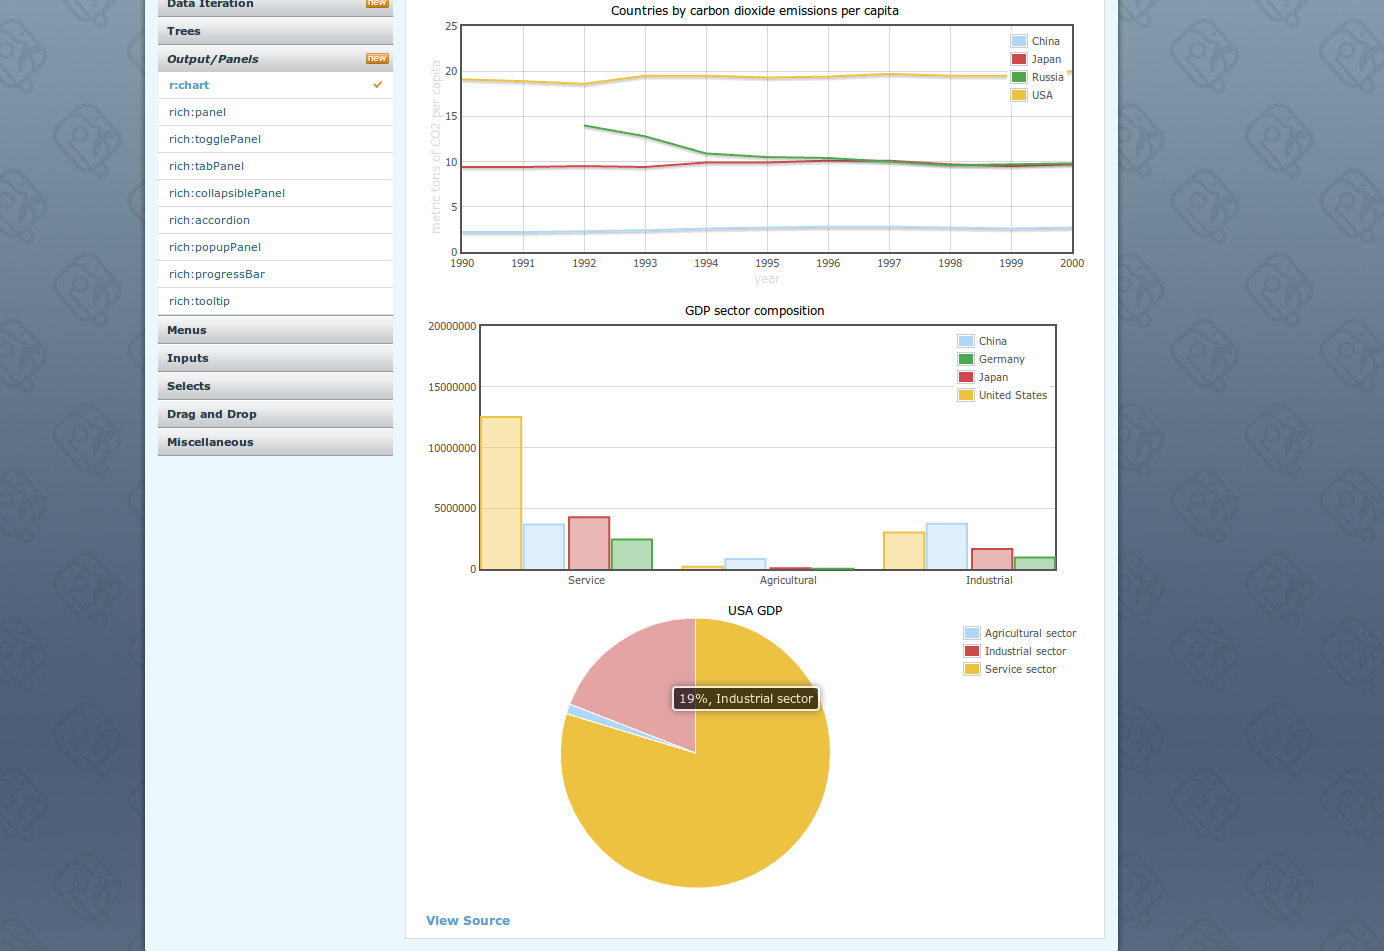
\includegraphics[width=0.9\textwidth]{figures/RichFacesShowcaseChartComponent.png}}}
    \end{center}
    \caption{RichFaces chart component shown in Showcase application}
    \label{fig:richfaces_chart} 
  \end{figure*}
  
  \section{Need for automation}
  The chapter \ref{sec:visual-testing-in-release-process} tried to outline how tedious and error prone might manual visual testing be. From our experience in the RichFaces QE team, any activity
  which needs to be repeated, and does not challenge tester's intellect enough, become a mundane activity. The more one repeats the mundane activity, the more likely an mistake is introduced:
  one forgets to try some use cases of an application, overlooks some minor errors, etc.
  
  Automated visual testing addresses this shortcomings, as it would unburden human resources from mundane activities such as manual testing, and would allow spending their
  time on intellectually more demanding problems. However, it introduces another kind of challenges, and needs to be implemented wisely. Following are minimal requirements 
  for a successful deployment of an automated visual testing.
      
  \section{Requirements for automation}
  \label{sec:requirementsForAutomation}
  An overall cost of the automation has to be taken into consideration. It is necessary to take into account higher initial cost of automation, and consequences it brings: 
  such as increased time to process relatively huge results of testing, cost of test suite maintenance.
  
  Therefore, to foster an effectiveness in quality assurance teams, while keeping the cost of automation reasonable low, automated visual testing would require:
  \begin{enumerate}
   \item A low cost of a test suite maintenance;
   \item a low percentage of false negative or false positive tests results;
   \item a reasonable time to execute the test suite;
   \item a concise yet useful test suite output;
   \item a support for Continuous Integration systems\footnote{Continuous Integration (CI) system is software to facilitate a practice of CI, which in short is about merging 
	  all developer copies with a shared mainline several times a day [5].}.
  \end{enumerate}
  
    \subsection{Low cost of test suite maintenance}
    A test suite needs to reflect a development of an application under test. Therefore, with each change in the application, it is usual that the test suite has to be changed as well.
    Making a change in the test suite can often introduce a bug, and cause false negative or false positive tests results.
    
    To keep this cost as low as possible, the test suite script has to be readable and meaningful, so when the change is about to be introduced, it is clear where and how it should be done.
    
    A test framework in which the test suite is developed should provide high enough abstraction. That would enable better re-usability for various parts of the test suite, 
    while lowering the overall cost of maintenance.
    
    Specifically for visual testing, when done by comparing screen captures, it is very important how well a repository of screen captures is maintainable. Secondly, 
    how reference (those correct ones, other screen captures will be compared with) screen captures are made.
    
    \subsection{Low percentage of false negative or false positive results}
    False negative test results incorrectly indicate a bug in an application under test, while it is a bug in the test suite itself. They are unwanted phenomenon as they take time to process
    and assess correctly.
    
    False positive tests results hide actual bugs in an application. They provide an incorrect feedback by showing the tests as passing, even when there is a bug in the application.
    
    Specifically for visual testing, when it is done by comparison of screen captures, it is very easily to be broken by small changes on a page. For example if the page outputs a current
    date, then it would break with every different date. There has to exist techniques, which would prevent these situations.
    
    \subsection{Reasonable time to execute a test suite}
    Reasonable time is quite subjective matter, but in general, it depends on how many times e.g. per day one needs to run whole test suite. Nowadays trend is a Continuous Integration,
    when a developer or a tester commits changes of an application several times per day to a shared source code mainline. Each such commit should trigger the test suite, which verifies 
    whether the change did not introduced an error to the application.
    
    According to creators of Continuous Integration practice, the whole point of CI is to provide a rapid feedback. A reasonable time for them is 10 minutes. If the build
    takes more time, every minute less is a huge improvement (considering a developer/tester runs test suite several times a day).
    
    \subsection{Concise yet useful test suite output}
    One of drawbacks of automated testing is its ability to produce huge amount of logs, test results etc. The output therefore needs to be as concise as possible, while still providing
    an useful information. A tester needs to be able to quickly recognize where the issue might be. The best situation would be if the tester does not need to run the test again in order
    to spot the issue. The output should give him a clear message where the issue is.
    
    For visual testing specifically, this can be achieved by providing a tester with screen captures together with difference of old and new version.
    
    \subsection{Support for Continuous Integration systems}
    This is quite easily to be achieved, but still, a developer of a tool for visual testing should have this in mind beforehand. Todays CI systems support variety of build systems, for
    various platforms, and languages. For example Jenkins supports build systems like Maven or Gradle, but it can run also shell scripts.
    
    
\chapter{Analysis of existing solutions}
\label{chap:analysis}
As we introduced in \ref{sec:requirementsForAutomation}, there are many aspects which need to be taken into consideration when automating visual
testing. Following analysis is going to compare existing solutions to automated testing with those requirements in mind, while introducing
different approaches to visual testing.

The representative list of tools for comparison was made also according to an ability to be used in enterprise context. In an enterprise company, there
is a stress on stability and reliability of employed solutions. It is quite vague requirement, and it is usually hard to find out which tools
are a good fit for enterprise companies, however, some indicators, which we used as well, might be helpful:
\begin{itemize}
 \item Is a project actively developed? When was the last release of the project, or how old is the last commit to a source code mainline?
 \item How many opened issues the project has? When was the last activity \\* with those issues ?
 \item What is the quality of the source code? Is it well structured? Does it employ best development practices?
 \item Does the project have a user forum? How active are the users?
 \item Is a big enterprise company behind the solution, or otherwise sponsoring it ?
 \item What are the references if the project is commercialized ?
\end{itemize}

For each tool in following sections we are going to show an example usage and its main drawbacks together with some basic description.
  
  \section{Mogo}
  Mogo [6] approach to visual testing can be in short described like: 
  \begin{enumerate}
   \item One provides set of URLs of an application under test to a cloud based system.
   \item Application URLs are loaded in various browsers, detection of broken links is done.
   \item Screenshots are made and are compared with older screenshots from the same URL to avoid CSS regressions.
  \end{enumerate}
  
  There is no programming script required, therefore it can be used by less skilled human resources. It can be configured in shorter time, and thus is less expensive.
  
  \subsection{Mogo drawbacks}
  
  Drawbacks of this approach are evident when testing dynamic pages, which content is changed easily. Applications which provide rich interaction options to an end user, and which state
  changes by interacting with various web components (calendar widget, table with sorting mechanism etc.), require more subtle way of configuring what actions need to be done before the
  testing itself. Mogo is suitable for testing static web applications, not modern AJAX enabled applications full of CSS transitions.
  
  Above mentioned drawbacks might lead to a bigger number of false negative test results when used with real data (any change, e.g. showing actual date may break testing), or to a bigger 
  number of false positive tests results when such a tool is used to test mocked data \footnote{Mocked data is made up data for purpose of testing, so it is consistent and does not 
  change over time}.
  
  \section{BBC Wraith}
  Wraith is a screenshot comparison tool, created by developers at BBC News [7]. Their approach to visual testing can be described like:
  \begin{enumerate}
   \item Take screenshots of two versions of web application by scripting either PhantomJS \ref{subsec:phantomJS}, or SlimerJS\footnote{SlimerJS is 
   very similar to PhantomJS \ref{subsec:phantomJS}, it just runs on top of Gecko engine, which e.g. Mozilla Firefox runs on top of. [10]} by another JavaScript framework called 
   CasperJS \ref{subsec:casperJS} [20].
   \item One version is the one currently developed (which run on localhost\footnote{In computer networking, \texttt{localhost} means this computer. [11]}), and the other one is a live site.
   \item Once screenshots of web page from these two different environments are captured a command line tool \texttt{imagemagic} is executed to compare screenshots.
   \item Any difference is marked with blue color in a created picture, which is the result of comparing two pictures (It can be seen at Figure \ref{fig:bbcWraithDiff}).
   \item All pictures can be seen in a gallery, which is a generated HTML site (It can be seen at Figure \ref{fig:bbcGallery}).
  \end{enumerate}
  
  To instruct BBC Wraith tool to take screenshots from the web application, one has to firstly script PhantomJS or SlimerJS to interact with the page, and secondly, creates a 
  configuration file, which will tell the PhantomJS instance which URLs need to be loaded and tested. PhantomJS script is one source of distrust to this tool, and therefore is
  introduced furthermore.
  
    \subsection{PhantomJS}
    \label{subsec:phantomJS}
    PhantomJS [8] is stack of web technologies based on headless\footnote{Headless software do not require graphical environment (such as X Windows system) for its execution.} 
    WebKit\footnote{WebKit is a layout engine software component for rendering web pages in web browsers, such as Apple's Safari or previously a Google Chrome [9]} engine, which can be 
    interacted with by using of its JavaScript API.
    
    For the sake of simplicity we can say that it is a browser which does not make any graphical output, which makes testing with such a engine a bit faster and less computer resources 
    demanding.
    
    One can instruct PhantomJS to take a screenshot of a web page with following script:
  
    \begin{verbatim}
      var page = require('webpage').create();
      page.open('http://google.com/', function(status) {
        if(status === 'success') {
          window.setTimeout(function() {
            console.log('Taking screenshot');
            page.render('google.png');
            phantom.exit();
          }, 3000);
        } else {
          console.log('Error with page ');
          phantom.exit();
        }
      });
    \end{verbatim}
    
    When executing such a script it will effectively load \texttt{http://google.com/} web page, waits 3000 milliseconds, and after that, creates a screenshot to the file \texttt{google.png}.
    
    In most environments it will be sufficient to wait those 3000 milliseconds in order to have the \texttt{www.google.com} fully loaded. However, in some resource limited environments, 
    such as virtual machines\footnote{Virtual machines are created to act as real computer systems, run on top of a real hardware}, it does not have to be enough. 
    It will result in massive number of false negative tests. There is a need for more deterministic way of finding out whether the page was loaded fully in given time, and 
    taking of the screenshots itself can take place.
    
    Another problem we noted in the previous script, is its readability. It is written in a too low level way (one has to control HTTP status when loading a page). Secondly, there is a need
    to explicitly call \texttt{page.render('google.png');} in order to take a screenshot. Script which would test a complex web application would be full of such calls. Together with poor
    way of naming created screenshots (a user has to choose name wisely), it might lead to problems when maintaining such a test suite.
    
    PhantomJS API is wrapped by CasperJS, which is furthermore described below.
    
    \subsection{CasperJS}
    \label{subsec:casperJS}
    CasperJS is navigation scripting and testing utility written in JavaScript for the PhantomJS and SlimerJS headless browsers. It eases the process of defining a full navigation scenario 
    and provides useful high-level functions for doing common tasks [20].
    
    Following code snippet shows a simple navigation on Google search web page. It will load \textit{http://google.com} in a browser session, 
    will type into the query input string \textit{MUNI}, and will submit it.
    
    \begin{verbatim}
    casper.start('http://google.com/', function() {
      // search for 'MUNI' from google form
      this.fill('form[action="/search"]', { q: 'MUNI' }, true);
    });
   
    casper.run(function() {
      this.exit();
    });
    \end{verbatim}
    
    The problem with this script, which we identified, is its low-level abstraction of the browser interactions. It makes tests less readable, and thus more error prone when a change
    is needed to be introduced.
    
    \begin{figure*}[!htb]
    \begin{center}
    \leavevmode
    \centerline{\scalebox{1.0}{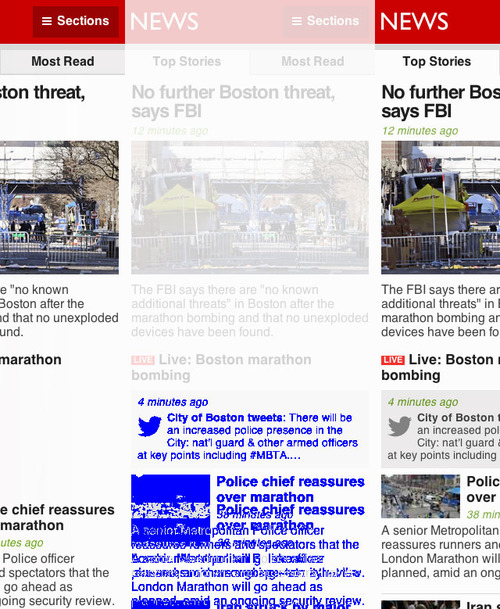
\includegraphics[width=0.4\textwidth]{figures/bbcWraith.jpg}}}
    \end{center}
    \caption{BBC Wraith picture showing difference in comparison of two web page versions [12]}
    \label{fig:bbcWraithDiff} 
  \end{figure*}

  
  \begin{figure*}[!htb]
    \begin{center}
    \leavevmode
    \centerline{\scalebox{1.0}{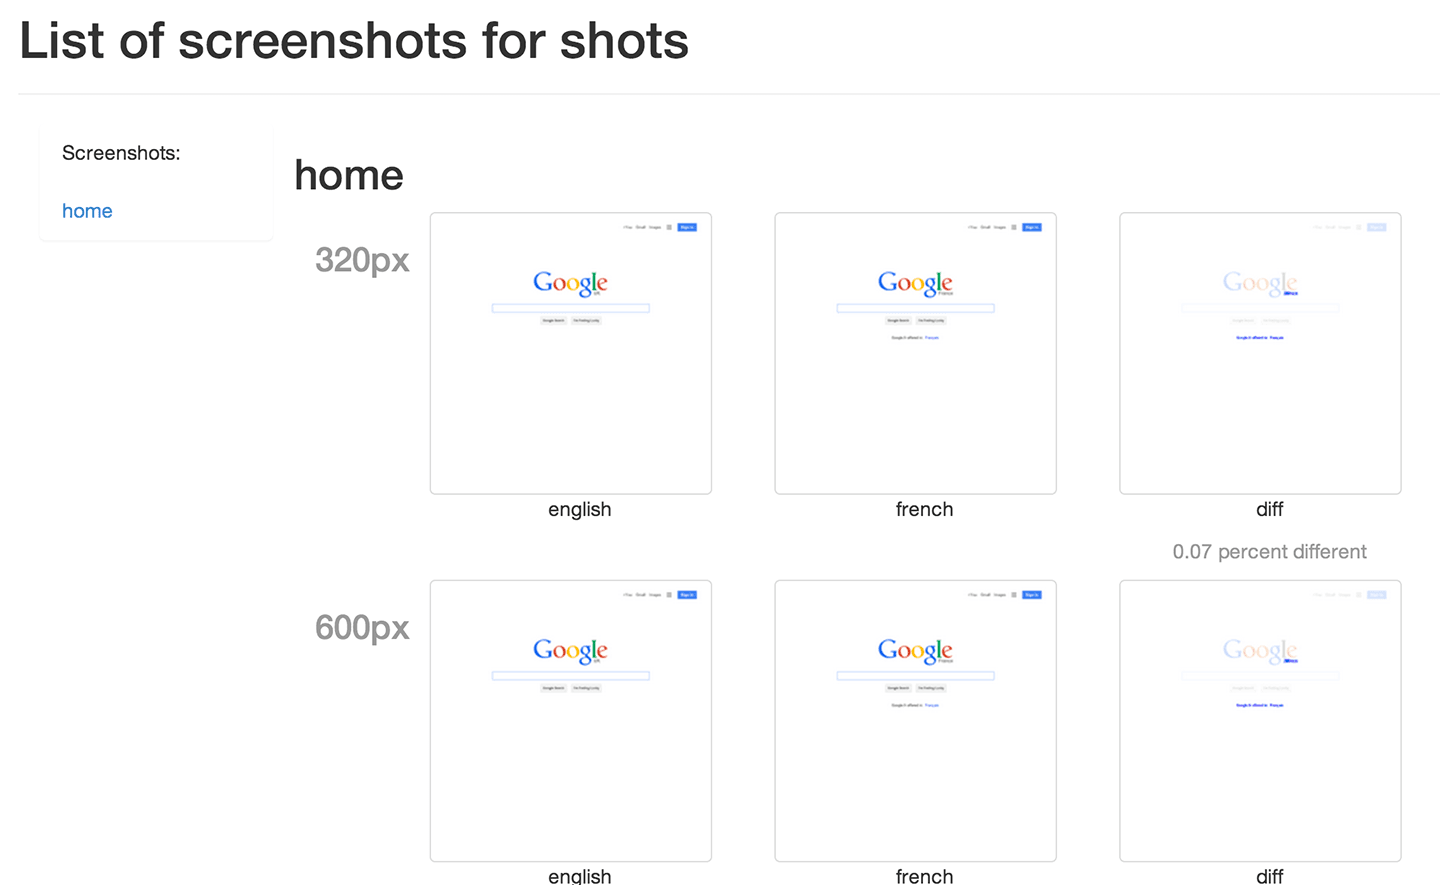
\includegraphics[width=0.8\textwidth]{figures/wraithGalleryExample.png}}}
    \end{center}
    \caption{BBC Wraith gallery example [13]}
    \label{fig:bbcGallery} 
  \end{figure*}

    \subsection{BBC Wraith drawbacks}
    Two of the drawback were described in the previous sections, \ref{subsec:phantomJS} and \ref{subsec:casperJS}.
    
    Another problem which might occur when testing with BBC Wraith, is cross browser compatibility. As it supports only PhantomJS, and therefore, one can not assure that the page will be 
    looking the same in all major browsers. The incompatibility comes from the fact, that browsers interpret CSS rules differently, and because they have different JavaScript engines. 
    Thus for example web page might look differently in Google Chrome and Microsoft Internet Explorer, and PhantomJS will not catch this issues.

  \section{Facebook Huxley}
  Another visual testing tool [15], supported by a big company Facebook, Inc. [14], uses similar approach in terms of comparing taken screenshots. The process of taking them, and the process
  of reviewing results is different though.
  
  \begin{enumerate}
   \item One creates a script which would instruct Huxley tool, what web pages screenshots should be taken from. Such a script might look like:
  
    \begin{verbatim}
      [test-page1]
      url=http://localhost:8000/page1.html

      [test-page2]
      url=http://localhost:8000/page2.html
   
      [test-page3]
      url=http://localhost:8000/page3.html
    \end{verbatim}
    
    \item One runs Huxley in the Record mode. That is the mode when Huxley loads the pages automatically in a fresh browser session, and a tester by hitting Enter keyboard button instructs 
    Huxley to take a screenshot. Screenshots are stored in a folder with test name (one given in the square brackets in the example above), together with a 
    JSON\footnote{JSON stands for JavaScript Object Notation, a standard format that uses human readable format to transmit data objects [16]} file describing mainly how long should 
    Huxley wait, when doing visual comparison, to have a tested web page fully loaded. Time is measured during this record mode.
    
    \item To start visual testing, one has to run Huxley in the Playback mode. Huxley will start fresh browser session, and will playback loading of the pages, with waiting for the pages
    to be fully loaded.
    
    \item When there is a change in an application, Huxley will log a warning, and takes a new screenshot automatically. In continuous integration environments, one can instruct Huxley
    to finish with error, in case screenshots are different. In that case, one can run Huxley again with an option to take new screenshots (if the change is desired, and is not an error).
   \end{enumerate}
    
   Main drawback of Facebook Huxley we can see, is similar to BBC Wraith, and that is its non deterministic approach to waiting for a fully loaded web page. It is again a fixed amount of time,
   which can be different from environment to environment. The time to wait can be configured, however, it is still quite error prone, as for first visual testing run
   e.g 4 seconds can be would be enough, and for another run would not.
    
   Secondly it lacks a proper way of viewing results of comparisons, leaving with only one option to check the command line output, together with manual opening of the screenshots. This would degrade
   cooperation among various QA team members, and it is harder to deploy in a software as a service cloud solutions\footnote{Software as a service is on demand software, centrally hosted, 
   accessed typically by using a thin client via web browser [17].}, where such a cooperation might take a place.

  \section{Rusheye}
  \label{sec:rusheye}
  Rusheye [18] is a command line tool, which is focused on automated bulk or on-the-fly inspecting of browser screenshots and comparison with predefined image suite. It enables automated
  visual testing when used together with Selenium 1 project [19].
  
  The process has subtle differences in comparison with previous solutions. It consists from these steps:
  
  \begin{enumerate}
   \item Screenshots are generated, for example by Selenium 1 tool, while functional tests of web application are executed.
   \item First screenshots are claimed to be correct (are controlled manually), they are called patterns.
   \item After a change in web application under test, another run of Selenium 1 tests generates new screenshots. They are called samples.
   \item Patterns and samples are compared, its visual difference is created, and result is saved in an XML file.
   \item The results can be viewed in a desktop application, Rusheye manager [22].
  \end{enumerate}
  
  Rusheye has one very important feature, which another tools lack. It is a possibility to add masks on particular parts of the screenshots. Those parts are ignored when two screenshots are
  compared. It is a huge improvement to protect from false negative tests, as some all the time changing parts (such as actual date, etc.) can be masked from comparison, and thus their change
  will not break testing.
  
  \subsection{Rusheye drawbacks}
  Core of the Rusheye is only able to compare screenshots generated by some other tool. Integration with Selenium 1 is advised, however, functional tests written in Selenium 1 suffer
  from the same problems [21] as scripts written for BBC Wraith \ref{subsec:casperJS}. And that is bad readability caused by their low level coupling with HTML and lack of higher abstraction.
  
  Another problem we can see is only a desktop version of the tool for viewing results (Rusheye Manager). Cooperation on some test suite among QE team members and developers would be 
  more difficult. As they would need to solve persistence of patterns, samples and descriptor of the test suite.
  
  \section{Conclusion of analysis}
  \label{chap:conclusion}
  All previously listed tools have some useful features, which we would like to be inspired with. However, all of the solutions lack something, what we suppose to be an inevitable part of 
  an effective automated visual testing.
  
  Figure \ref{fig:existingSolutionComparison} summarizes requirements we have for a visual testing tool, and the fact whether the tool satisfies the particular requirement.
  
  Tests readability is a problem we discussed with a particular tool description. It is a level of abstraction over underlaying HTML, in which the application is written. It is quite subjective
  matter, however, there are some clues by which it can be made more objective. For example the way how tests are coupled with the HTML or CSS code. Because the more they are, the less they 
  are readable [21]. A scale we used for evaluation supposes insufficient as lowest readability, which in long term run of the test suite might cause lot of issues.
  
  By tests robustness we suppose a level of stability running of the tests with particular tool has. 
  It means how likely there are false positive and false negative tests, whether are caused by not fully loaded page, or by dynamic data rendered on the page. If the robustness is low,
  you can find a red mark in a particular cell. Green one otherwise.
  
  Cross browser compatibility issue deals with ability to test web application across all major browsers \ref{footnote:majorBrowsers}.
  
  By cloud ready features we suppose whether tool has web based system for reviewing results, and thus enables cooperation across QA team members and developers of the particular software.
  
  Continuous Integration friendliness in this context means the fact whether tool is suitable for usage in such systems. It actually means whether output of the tool is clear enough,
  how much work a tester would be required to do manually to deploy such a tool in a test suite. Whether testers would need to review just logs to find visual testing failure, or
  whether it will be somehow visible, e.g. whole test would fail.
  
  \begin{figure*}[!htb]
    \begin{center}
    \leavevmode
    \centerline{\scalebox{1.0}{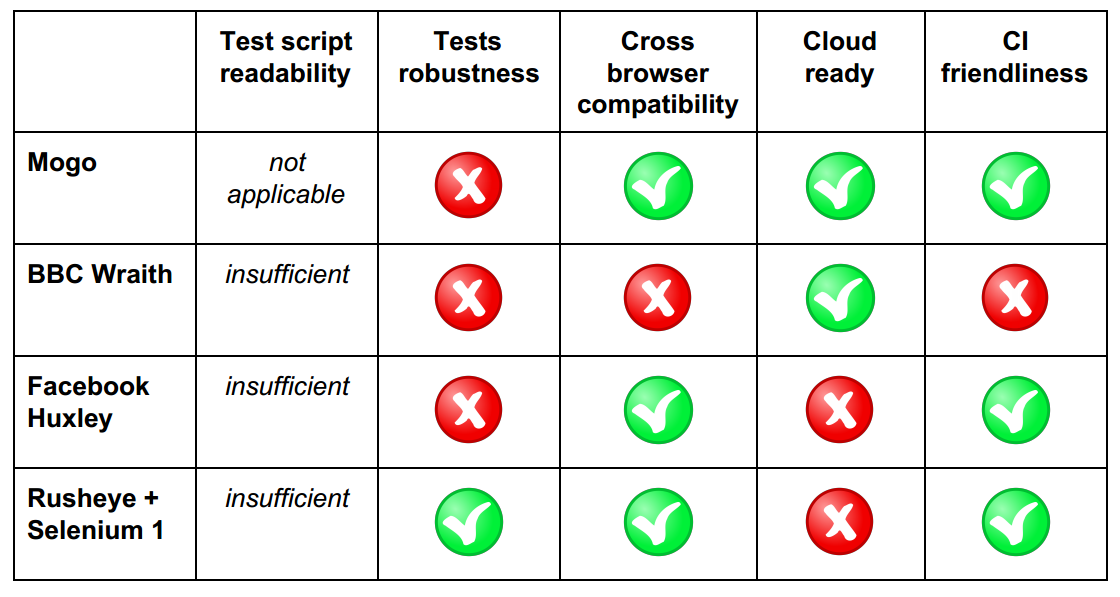
\includegraphics[width=0.8\textwidth]{figures/existingSolutionsTableComparison.png}}}
    \end{center}
    \caption{Existing solutions features comparison}
    \label{fig:existingSolutionComparison} 
  \end{figure*}
  
  As Figure \ref{fig:existingSolutionComparison} shows, none of the tools met our requirements fully. Therefore, we decided to proceed with developing of a new tool, which would address
  all issues, and which would integrate existing parts of the solutions when it is reasonable. Creation of a new process which would enable effective usage of such
  tool by QA team members is inevitable. Following chapters describe this new tool and the new process.
  
\chapter{New approach}
  Each tool by its definition introduces a process for a visual testing. While we recognized shortcomings (described in the chapter \ref{chap:conclusion}), we realized a need for a different 
  approach to the visual testing. The approach came from 2 and half years of developing and maintaining the functional test suite \footnote{The RichFaces test suite is available at 
  https://github.com/richfaces/richfaces-qa} for RichFaces project \footnote{RichFaces is component library for Java Server Faces web framework [23]}.
  
  \section{Hypothesis}
  \label{sec:hypothesis}
  It should be enough to have just a functional test suite for a end to end testing of an application. Scripts from functional testing interacts with the application sufficiently, 
  therefore, another script which during such interactions take screenshots is redundant.
  
  This redundancy is expensive, because quality assurance teams need to maintain more test suites. A change in the application needs to be introduced on more places, which allows errors to
  sneak in test suites.
  
  In the same time we do believe, that script for functional testing should be abstracted from a visual testing as much as possible. Meaning that, explicit calls to methods which 
  take screenshots, should be optional. Functional test script should take screenshots automatically during testing, in each important state of an application. By this, we will achieve better
  readability of the functional tests' scripts.
  
  For sure there should be an option to make screenshots explicitly, however, a need to facilitate such option should be sporadic. This will be achieved by fine-grained configuration options.
  A tester should be able to to configure on global level, meaning for all tests from one place, as well as on test level, in what situations a screenshot should be taken.
  
  The base of screenshots which will serve as a reference for a correct state of the web application, will be made automatically during first run of the created tool. 
  Screenshots should be made available automatically for all interested parties (developers, testers, etc.).
  
  A viable solution seems to be introducing a web interface, as a system for managing results of visual testing comparison. In this system (called a manager in this thesis), a user should be
  able to decide about results of visual testing. More particularly asses the results, whether there is a bug in application or not. 
  This web interface will foster cooperation between interested parties.
  
  By following above mentioned principles, we will achieve a better effectiveness of a quality assurance team. More particularly we will massively decrease amount of time they need to spend 
  with manual testing.
  
  \section{Process}
  \label{sec:process}
  The whole solution for visual testing would need to include reaction on these problems:
  \begin{enumerate}
   \item Executing a visual test suite for the first time to generate patterns, which are new screenshots in subsequent tests executions will be compared with.
   \item Executing the visual test suite for second and more times, to generate new screenshots, which are called samples in this thesis, for comparison with patterns generated in the fist run.
   \item Review results, and take an action when there is a false negative result, or bug in the application.
   \item Executing the visual test suite when a new test is added, deleted, or otherwise changed.
  \end{enumerate}

  For simplicity, in the first stage of development, we suppose the third problem to be solved with re-executing the whole test suite
  again, as it is done in the first run of the test suite. Overall process can be described with following subprocesses.
  
  \subsection{First execution of functional tests}
  \label{chap:firstRunProc}
  
  Figure \ref{fig:FirstTestsRunBMPN} denotes steps needed to generate patterns. It is a prerequisite for the visual testing.
  
  Screenshots are generated during execution of the tests. If all functional tests pass, those screenshots
  can be claimed as patterns, and are uploaded to a storage. Screenshots generated in tests which failed, are ignored, they are
  not included in the visual testing. Such functional test need to be fixed, made to be passing, to include it to visual testing.
  
  An optional part is reviewing of the screenshots. If there is any issue with patterns, they should be thrown away, and tests will be rerun.
  
  If patterns are correct, a tester can proceed with subsequent runs of the test suite to start the actual visual testing.
  
  \subsection{Subsequent execution of visual testing}
  
  Figure \ref{fig:NextTestsRunsBMPN} shows how subsequent execution of visual testing together with functional testing would look like. The first step is same as in previous process,
  functional tests are executed, and screenshots are taken. Secondly, patterns are downloaded from the storage, and after that actual visual testing can start.
  
  Newly created screenshots, called in this thesis samples, are pixel to pixel compared with downloaded patterns. Result is stored in a descriptor file, and differences between particular
  pattern and sample are visually stored in a generated picture.
  
  If there are found some differences, generated pictures together with their corresponding samples, and patterns are uploaded to a remote storage.
  
  Users should be able to review the results from now on, where he will find the particular run according to a time stamp when the run was executed. They should be able to asses the results,
  with displayed triplet, consisting of patter, sample and their difference. They should be able to say whether it is false negative test result, in which case they should be able to 
  take an action to prevent such results in the future. One of such actions can be applying masks, which is more described in chapter \ref{sec:rusheye}.
  
  The tool should be configurable, so such false negative results are rather sporadic, instead, failed visual comparison tests should reveal a bug in the application under test. In that case
  it is in user responsibility to file such a bug in a corresponding issue tracker. Generated pattern, sample and difference can be used as a useful attachment to a issue report, which
  would better describe actual and expected result.
  
   \begin{figure*}[!htb]
    \begin{center}
    \leavevmode
    \centerline{\scalebox{1.0}{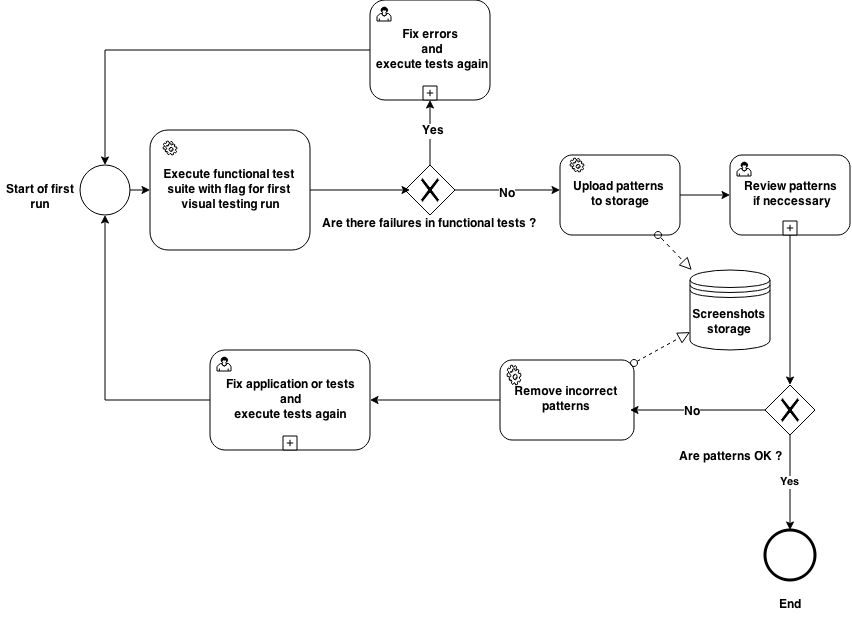
\includegraphics[width=1.0\textwidth]{figures/FirstTestsRunBMPN.png}}}
    \end{center}
    \caption{Process to generate patterns during first execution of functional tests.}
    \label{fig:FirstTestsRunBMPN}
  \end{figure*}
  
  \begin{figure*}[!htb]
    \begin{center}
    \leavevmode
    \centerline{\scalebox{1.0}{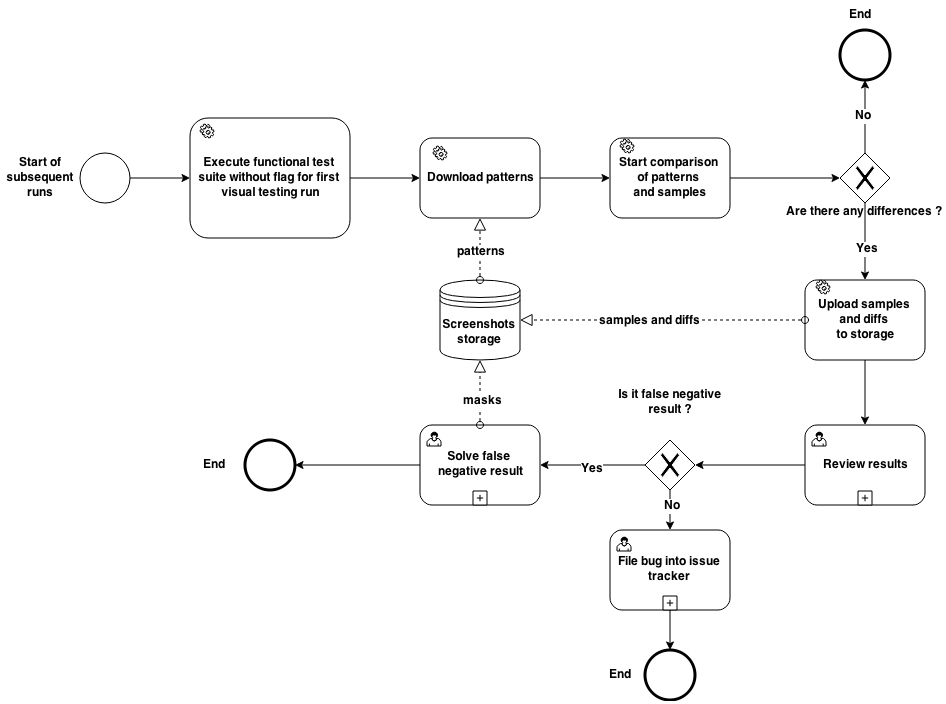
\includegraphics[width=1.0\textwidth]{figures/NextTestsRunsBMPN.png}}}
    \end{center}
    \caption{Subsequent execution of visual testing together with functional tests.}
    \label{fig:NextTestsRunsBMPN}
  \end{figure*}
  
  \newpage
  \section{Analysis of useful tool output}
  \label{sec:analysisUsefulOutput}
  To create a tool, which is widely accepted by a community of testers, who are interested in a visual testing, we have to take usefulness of the tool as a priority. Such tool has to show results
  of the visual comparison in a way, that it is a pleasure to use it. In the end of the day, the amount of time spent with using of the tool has to be dramatically less than doing the manual
  visual testing.
   
  Therefore, we conducted a research among IT experts, which took a form of brainstorming on the visual testing web application user interface. Purpose of such a web application is to show
  results and allow a tester to take an immediate action over them.
  
  The brainstorming took place on Arquillian developer forum [24], which is daily accessed by hundreds of users. By the time of writing of this thesis, it has more than 355 views, 
  and 11 replies. We can say that there are users interested in such a tool, and we have gained a valuable feed back, together with many interesting ideas what features such a web application
  for reviewing results should have.
  
  We started with description of tool together with proposals for graphical user interface design (mockups), and asked IT community for their
  opinions, what they miss on such interface, what is on the other hand redundant.
  
  You can see created mockups in appendix \ref{appendeix:a}. The web application is logically divided into
  three screens. First one (can be seen in appendix \ref{fig:frontPageMock}) is showing front page of the application. Its purpose
  is to show test suites, which are groups of tests written for a particular application under test.
  Together with a web browser they are tested on, represent a test suite for visual comparison testing.
  
  Second screen (can be seen at \ref{fig:particularRunMock}) shows a particular executions of the test suite. These test
  suite runs are unambiguously named according to a time and date, they were executed.
  
  Third created mockup shows comparison results for a particular tests suite run. The comparison result
  consists from three screenshots. A pattern, created during first run of the test suite. A sample, which
  was taken during this particular test execution, and a picture called diff, which denotes differences
  between the pattern and the sample.
  
  On the third mockup you can also see two buttons. They purpose is to allow a tester to take an immediate
  action upon results. Pattern is correct button, is used when the result of the comparison is
  a false negative, or when the result denotes a bug in the application. Sample is correct button, is used
  when there is an anticipated change in the application under test. 
  In that case the new created sample should be used as the pattern in next comparisons.
  
  Based on users insight, we complemented the final web application with following features:
  
  \begin{itemize}
   \item Indicate number of failures versus total number of tests.
   \item Revision number of application under test. For example Git\footnote{Git is source code version system, http://git-scm.com/}
   commit id.
   \item Display together with screenshots also the name of the functional test, and a name of the test class
   the test resides in.
   \item The triple pattern, sample, diff should be displayed in a way that it is not hard to spot the
   actual difference. Putting them side by side is not a good option. We had to think out some different
   approach.
   \item Together with time stamp of the run, we should also show an order number of the run.
  \end{itemize}

  
\chapter{Implemented tool}
To support our hypothesis and the process we figured out, a set of tools needed to be created. As we did
not want to reinvent a wheel, where it is feasible we used already existing tool, and integrated it to the
final result.

Figure \ref{fig:componentDiagramOfImpl} depicts component diagram of implemented solution. It is only a high
level picture of overall solution. Particular components are described in detail in following chapters.

\begin{figure*}[!htb]
    \begin{center}
    \leavevmode
    \centerline{\scalebox{1.0}{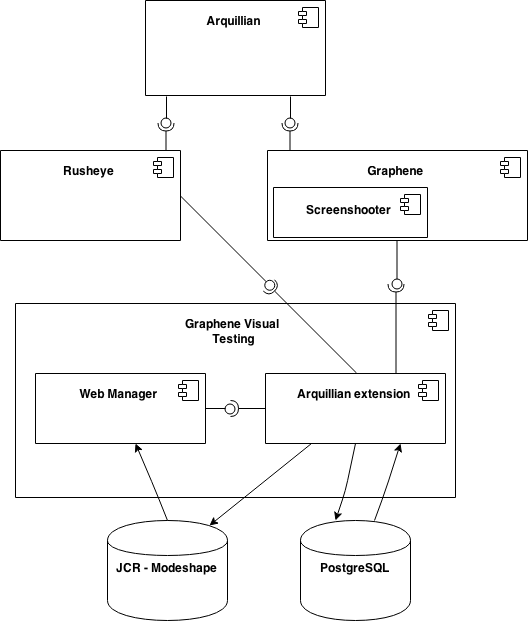
\includegraphics[width=0.7\textwidth]{figures/VisualTestingComponentDiagram.png}}}
    \end{center}
    \caption{Component diagram of implemented solution for visual testing.}
    \label{fig:componentDiagramOfImpl}
\end{figure*}
  
\section{Arquillian}
Arquillian\footnote{More information about Arquillian at http://arquillian.org/} is a testing framework, which facilitates integration testing. It automatizes various parts
of the integration testing, which allows testers to develop actual tests.

It can for example: start application container before testing, and to stop it after tests execution 
is done, can deploy application under test to that container, populate database with testing data, 
start web browsers, test on mobile devices, and to provide useful output with videos and screenshots 
from testing.

In other words, it manages life cycle of all integration components your application integrate with.

It has very nice architecture, which resembles an event based machine. It is easily extensible, as it
supports Service provider interface pattern [25]. It can cooperate with all major browsers, which makes
it a cross browser solution. 

All these features made it a good candidate to integrate our solution with. We did not need to develop any
feature for this project.
  
\section{Arquillian Graphene}
Arquillian Graphene is an extension to Arquillian, thus fully supports its life cycle of test. Its main
purpose in integration tests is to control a web browser. By using its API, a tester is able to for example
click on the button on the web page, write some characters into text inputs or otherwise interact with
a web application under test.

Its core is a wrapper over well known project Selenium (also known as WebDriver) 
\footnote{More information about Selenium project at http://www.seleniumhq.org/}. It is a W3C 
standard\footnote{WebDriver working draft standard available at http://www.w3.org/TR/webdriver/},
which guarantees stability, making it a good candidate to build our solution with.

Graphene's type safe API\footnote{Type safe API in Java programming language enforces obeying various rules
before compilation of source code, thus decreases a change to introduce an error.} supports design patterns
such as Page Object\footnote{Page Object pattern encapsulates a web page into object, makes tests
more readable [26].} or Page Fragment\footnote{Page Fragments pattern divides a web page further into reusable 
components which encapsulates a web widget functionality, making tests more reusable and readable [27].}.

Those features form an API with hight abstraction level, and encourage a tester to develop more readable
tests. Those are attributes, which already existing solutions lack (see \ref{chap:conclusion} for more
information).

\section{Graphene screenshooter}
For the purpose of visual testing, we needed to implement one addition to Arquillian Graphene. 
A component which would facilitate taking of screenshots of application under test in a uniform manner.
Developed addition implement a common interfaces defined in Arquillian Recorder extension
\footnote{Arquillian Recorder is an extension which among the other things defines interfaces 
for screenshot taking, and video recording from tests executions. We have cooperated on defining this
common interfaces as well. More information at https://github.com/arquillian/arquillian-recorder}.

We had two main requirements on this screenshots taking extension, which came directly from the analysis of
already existing solutions (see chapter \ref{chap:analysis}):

\begin{enumerate}
 \item A tester should be able to configure this extension so it takes screenshots automatically. A script
 for functional test should be unaware of such screenshots taking behavior. It will stay clean and more 
 readable (see chapter \ref{chap:conclusion} to see more background information for this requirement).
 The configuration should be done on a global level, in other words for the whole test suite.
 \item The tester on the other hand should be able to explicitly enforce taking of screenshot at any place
 in the functional test script. This should be just an optional feature, used rather sporadically.
\end{enumerate}

Second point is developed in all existing solutions, to enhance readability we required from our solution
to have implemented also point number one.

The global configuration is done where all configuration take place for Arquillian framework. 
It is in \texttt{arquillian.xml} file.

\begin{lstlisting}[caption=Example of screenshooter configuration in arquillian.xml,label=lis:screenshooterconf,language=xml]
<extension qualifier="screenshooter">
  <property name="takeBeforeTest">true</property>
  <property name="takeAfterTest">true</property>
  <property name="screenshotType">PNG</property>
</extension>
\end{lstlisting}

In the example configuration \ref{lis:screenshooterconf}, you can see, that screenshots are automatically 
made after two events: before test, which is effectively just after the web application is loaded in 
a browser, and after the test. 

We also started with an experimental feature, which is not fully available, and that is an option
to take screenshots after every action made by Selenium in browser\footnote{See more information 
about \texttt{takeOnEveryAction} at https://github.com/arquillian/arquillian-graphene/tree/master/extension/screenshooter}.
  
\section{Rusheye}
We have already described some of the Rusheye features in chapter \ref{sec:rusheye}. Its important that it
is only a command line tool, so integration with such a tool would require either executing its binary,
packaged in a \texttt{.jar} file, or calling its main\footnote{Java main method is an entry point
to the program.} method. That is not a good software design, because it is hardly extensible, and error prone,
when there is a change introduced in either of the integrated parts.

Therefore, we decided to introduce an integration layer in Rusheye, which would cooperate with Arquillian event based system.
It is mostly realization of Observer pattern\footnote{Observer pattern - \url{http://en.wikipedia.org/wiki/Observer_pattern}}.

Rusheye observes to events like: \texttt{StartCrawlingEvent}, or \texttt{StartParsingEvent}, and reacts according to it. It starts
crawling of patterns, and creates a test suite descriptor (XML file which describes where are the particular screenshoots for a particular
functional test stored). This is done after first run only (see chapter \ref{chap:firstRunProc}). In subsequent runs \texttt{StartParsingEvent}
is fired, and Rusheye starts actual visual comparison, it compares patterns with samples on pixel to pixel basis.

After crawling or parsing is done, it fires \texttt{CrawlingDoneEvent} or \texttt{ParsingDoneEvent} events respectfully, so other integrated
modules can wire up.

In result, such event based architecture, makes a loosely coupled system, which is easily extensible.

\begin{lstlisting}[caption=Example of StartParsingEvent observer,label=lis:startParsingObserver,language=java]
public void parse(@Observes StartParsingEvent event) {
     // Initialization code ommited
     parser.parseFile(suiteDescriptor, event.getFailedTestsCollection());
     parsingDoneEvent.fire(new ParsingDoneEvent());
}
\end{lstlisting}
  
\section{Graphene visual testing}
    It is a project, which has two purposes.
    \begin{itemize}
     \item to integrate and control Rusheye with Arquillian;
     \item and to provide a way for reviewing results of visual comparison.
    \end{itemize}

    For those two purposes, two sub-projects were created, and are described bellow.
    
    \subsection{Arquillian extension}
    \label{sec:arqExt}
    As it was written previously, this extension is focused on controlling Rusheye, and storing or retrieving of created screenshots.
    
    As listings \ref{lis:afterSuiteObserverObserver} shows, it wires up to Arquillian life-cycle, as it listens to \texttt{AfterSuite} event. 
    If it is a first execution of test suite, then it just fires \texttt{StartCrawlingEvent} event, which is observed by Rusheye. 
    After crawling is done, it stores created suite descriptor, and screenshots to a Java Content Repository 
    (JCR - see chapter \ref{chap:storage}).
    
    If it is not a first run, it firstly downloads screenshots and the suite descriptor, and then fires a \texttt{StartParsingEvent}, 
    which is again observed by Rusheye.
    
    The result of parsing (XML file describing what patterns and what samples were different, and a path to created diffs) are also uploaded
    to a JCR.
    
    \begin{lstlisting}[caption=AfterSuite observer to controll Rusheye,label=lis:afterSuiteObserverObserver,language=java]
     public void listenToAfterSuite(@Observes AfterSuite event) {
        
        String samplesPath = scrConf.get().getRootDir().getAbsolutePath();
        
        if (visualTestingConfiguration.get().isFirstRun()) {
            crawlEvent.fire(new StartCrawlinglEvent(samplesPath));
        } else {
            String descAndPtrDir = serviceLoader.get()
                    .onlyOne(DescriptorAndPatternsHandler.class)
                    .retrieveDescriptorAndPatterns();
            
            startParsingEvent.fire(new StartParsingEvent(
		      descAndPtrDir,
		      samplesPath, failedTestsCollection.get())
		      );
        }
     }
    \end{lstlisting}
    
    A communication between this extension and a JCR is done via JCR Rest API. To issue a http request, we are using Apache HttpComponents
    project\footnote{Apache HttpComponents - \url{http://hc.apache.org/}}.
 
    \subsection{Web application to view results}
    \label{sec:webManagerAppDesc}
    It is a web application for reviewing for reviewing results, but also for an active changing
    of the visual testing configuration.
    
    The application back-end is developed with use of Java Enterprise Edition\footnote{Java Enterprise Edition - 
    \url{http://www.oracle.com/technetwork/java/javaee/overview/index.html}} stack.
    It includes using of technologies like: Java Persistence API 
    \footnote{JPA - \url{http://en.wikipedia.org/wiki/Java_Persistence_API}} plus 
    PostgreSQL\footnote{PostgreSQL database - \url{http://www.postgresql.org/}} for a persistence
    layer. Enterprise Java Beans\footnote{Enterprise Java Beans - \url{http://en.wikipedia.org/wiki/Enterprise_JavaBeans}} 
    for controllers code (Model-Viewer-Controller 
    pattern\footnote{Model-Viewer-Controller - \url{http://en.wikipedia.org/wiki/Model-view-controller}}).
    It exposes Java API for RESTful Services (JAX-RS\footnote{JAX-RS - \url{https://jax-rs-spec.java.net/}}) endpoints to communicate
    enable communication with Arquillian extension (see chapter \ref{sec:arqExt}), and with its client part (HTML front end) in a
    RESTful way.
    
    The application is deployed on a WildFly application server\footnote{WildFly application server - \url{http://www.wildfly.org/}}.
    We chose this server, because of its an open source software, backed with huge community of users, and by a big enterprise,
    Red Hat\footnote{Red Hat - \url{http://www.redhat.com/en}}. Very important for us was also its fastness and availability in
    cloud environments (see chapter \ref{sec:cloudReady}).
    
    The front end is developed with use of AngularJS, which is a MVC framework for creating a Single Page Applications 
    (SPA\footnote{SPA - \url{http://en.wikipedia.org/wiki/Single-page_application}}. It is complemented with Twitter Bootstrap
    framework, to provide a visually pleasant UI.
    
    The design of particular screens are in accordance with the analysis described in section \ref{sec:analysisUsefulOutput}.
    You can find screenshots from the application in the [DOPLNIT APPENDIX].
    
    For better convenience, and to verify possibility to deploy application on the cloud, we have
    deployed it on Platform as a Service, OpenShift by RedHat cloud\footnote{OpenShift by RedHat - \url{https://www.openshift.com/}}.
    \\* Please see chapter \ref{sec:cloudReady} for more information about the deployment (how to log in, etc.).
    
    Following figure \ref{fig:useCaseDiagramWebManApp} depicts possible use cases with the web application, to give a better picture what can be achieved
    with this application.
    
    The most important here are \texttt{Reject Pattern} and \texttt{Reject Sample} functionalities, as they allow a tester to react
    on results. \texttt{Reject Pattern} will change in the storage for all screenshots the pattern with sample. This functionality is
    used when there is an expected change in the application, and we want to use the new sample as pattern in subsequent runs.
    
    \texttt{Reject sample} is used when the results is either false negative (in which case the sample is just deleted, or when
    there is a bug in the application under test, in which case a tester is supposed to create a bug report. Created sample and diff
    will serve as a good help when describing the bug. 
    
    There are planned extensions to this basic functionality, described in section \ref{sec:plannedExtensions}.
    
    \begin{figure*}[!htb]
      \begin{center}
      \leavevmode
      \centerline{\scalebox{1.0}{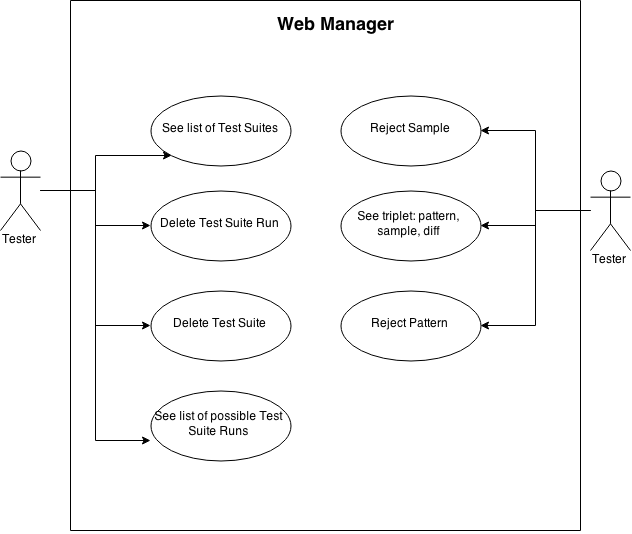
\includegraphics[width=0.7\textwidth]{figures/WebManagerUseCaseDiagram.png}}}
      \end{center}
      \caption{Use case diagram for Web Manager web application.}
      \label{fig:useCaseDiagramWebManApp}
    \end{figure*}
        
\section{Storage for images}
\label{chap:storage}
    As we had to think wisely when developing UI for Web Manager, to enable successful employing of the tool among community of 
    testers, the same we had to think beforehand about storage for created images (screenshots). 
    
    We have these requirements for storing of the images:
    
    \begin{itemize}
     \item The chosen solution has to provide way for storing large amount (hundreds) of pictures;
     \item it should be a scalable solution;
     \item it should provide a solid performance when uploading and downloading of stored pictures;
     \item it should be capable to ensure a security for data, authentication and authorization when accessing pictures;
     \item it should be a cloud friendly solution.
    \end{itemize}
 
    We were choosing from these options, which we choose by a careful analysis of patterns:
    \begin{enumerate}
     \item Store screenshots as Binary large objects (BLOBs 
	   \footnote{BLOB - \url{http://en.wikipedia.org/wiki/Binary_large_object}}) in a relational
	   database, such as PostgreSQL.
     \item Store screenshots in a file hosting service such as Dropbox\footnote{Dropbox - available at \url{https://www.dropbox.com/}}, 
     or Google Drive\footnote{Google Drive - available at \url{https://www.google.com/drive/}}. Store just URLs to relational database.
     \item Store screenshots in a Java Content Repository (JCR\footnote{JCR - specification available at 
	   \url{https://jcp.org/en/jsr/detail?id=283}}). Store just URLs to relational database.
    \end{enumerate}

    The number one option, has some obvious advantages. Databases are a superior solution where transactional integrity between the
    image and metadata are important. Because, it is more complex to manage integrity between database metadata and file system data, 
    and within context of a web application, it is difficult to guarantee that data has been flushed to disk on the file system [28].
    
    However, the way to store pictures in database as BLOBs, has some disadvantages too: database storage is usually more expensive
    than file system storage; database access can not be accelerated for example by configuring a web server to use system call to
    asynchronously send a file directly a network interface, as it can be done for file system access [28].
    
    Option number two seems to be a viable solution for smaller test suites. It does not suffer from the problems which database does.
    In a later stage of development of our tool we would like to provide this option to users of our tool. For now, we would like to
    provide more flexible solution, which does not vendor lock in to some providers. Which is free of charge when big storage
    space is required.
    
    Therefore, we chose option number three as pilot way for storing screenshots. JCR is a specification, and also a Java
    API, thus a best fit for our Java based application. We liked what kind of data and access
    patterns JCR are very good at handling [29]:
    
    \begin{itemize}
     \item Hierarchical data;
     \item files;
     \item navigation-based access;
     \item flexible data structure;
     \item and transactions, versioning, locking.
    \end{itemize}
    
    Data we need to store is naturally hierarchical. See figure \ref{fig:ourJCRHierarchy} to 
    see in what hierarchy we need to store generated screenshots, XML suite descriptor, and XML result descriptor (configuration
    files for Rusheye module).
    
    JCR are good at storing files, this is exactly what we are looking for, as pictures will be the main artifacts which we need to
    persist.
    
    Navigation based access is often used for application dealing with hierarchical data. In our application we need to work often 
    only with subset of the hierarchy - for example display triplet pattern, sample, and diff for a particular test suite run.
    
    We wanted to provide flexible data structure. By this tool stays extensible to other approaches and new features for later
    development (see section \ref{sec:plannedExtensions}).
    
    Transactions, versioning, and locking are sweet points which will be used in later development. They are important, as we want
    our solution to be scalable 
    (scale out\footnote{Horizontal scaling (scale out) - \url{http://en.wikipedia.org/wiki/Scalability}}),
    and we want to allow cooperation of testers on a particular test suite (their actions on results will need to be transactional).
    
    \begin{figure*}[!htb]
      \begin{center}
      \leavevmode
      \centerline{\scalebox{1.0}{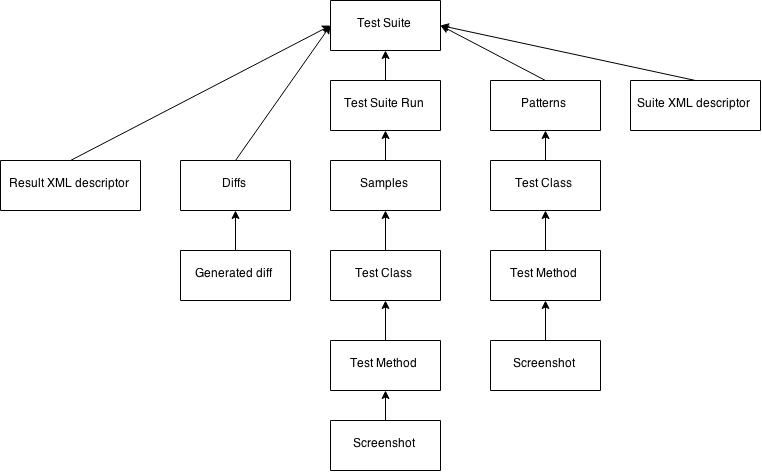
\includegraphics[width=1.0\textwidth]{figures/HierarchyJCR.png}}}
      \end{center}
      \caption{The hierarchy of nodes in our JCR deployment.}
      \label{fig:ourJCRHierarchy}
    \end{figure*}
    
    \label{sec:whyWeChooseJCR}
    We chose JCR implementation ModeShape\footnote{JBoss ModeShape by Red Hat - \url{http://modeshape.jboss.org}}. There are number
    of advantages we saw, when comparing this implementation with reference implementation of JCR, the Apache 
    Jackrabbit\footnote{Apache Jackrabbit - \url{http://jackrabbit.apache.org}}: The development is backed by Red Hat, the same 
    company we chose the application server from (see \ref{sec:webManagerAppDesc}). 
    They cooperate well with each other, and there is plenty of documentation on how to integrate those two systems.
    ModeShape also by default exposes a RESTful API for accessing and modifying the content of the repository. We are utilizing 
    this feature in the Web Manager (see \ref{sec:webManagerAppDesc}), when screenshots we want to display in the client browser,
    do not have to be firstly streamed to the WildFly application server, and then served to the client, but they are directly
    streamed to the client browser, as it knows the URL of the screenshot.
    
    For the future development we like its support for 
    WebDAV protocol\footnote{WebDAV protocol - \url{http://en.wikipedia.org/wiki/WebDAV}}, and possibility to cluster multiple
    ModeShape instances.
    
\chapter{Deployment of tool and process}
After implementing the tool, to prove or disprove hypothesis from section \ref{sec:hypothesis} we need to deploy the tool and the
process (see section \ref{sec:process}) on a real application. Following chapters describe such deployment, real world use cases
and best practices when using our tool.

To have a better picture, in what systems and environments, each part of the visual testing will be executed, following
sequence diagram was created:

\begin{figure*}[!htb]
      \begin{center}
      \leavevmode
      \centerline{\scalebox{1.0}{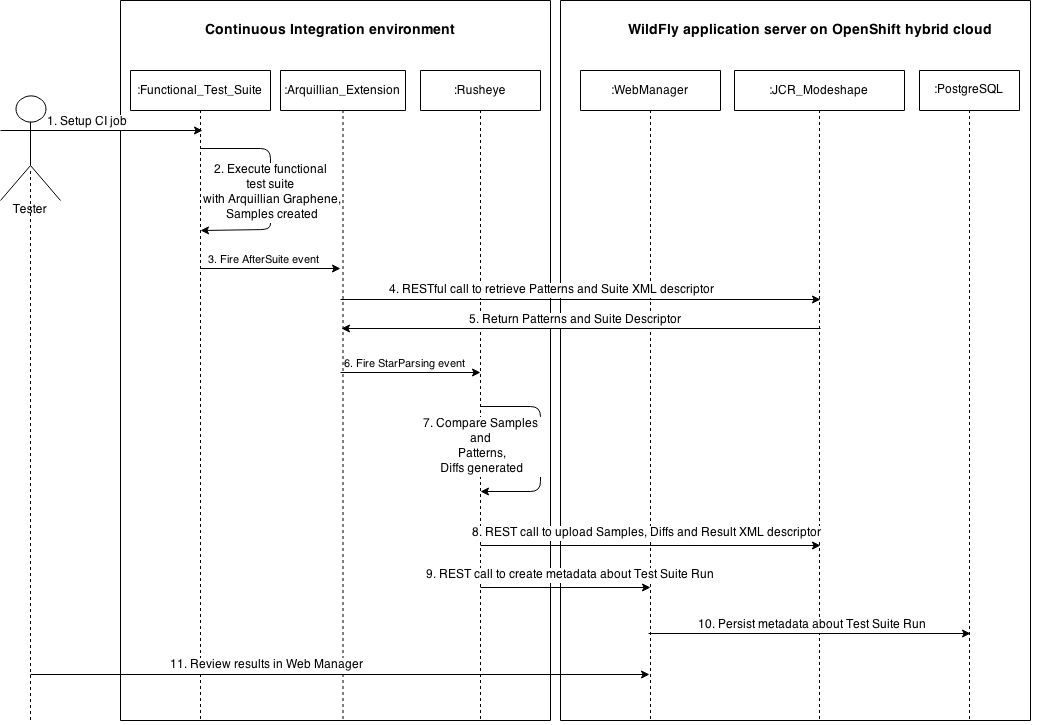
\includegraphics[width=1.0\textwidth]{figures/wholeSolutionSequenceDiagram.png}}}
      \end{center}
      \caption{Whole visual testing solution sequence diagram.}
      \label{fig:wholeSolutionSequenceDiagram}
\end{figure*}

There are omitted processes which are not important for visual testing, or processes which describes how data is transported into
the Web Manager, already described in section \ref{sec:whyWeChooseJCR}.
  
  \section{Actual visual testing}
  We chose RichFaces Showcase 
  application\footnote{RichFaces Showcase - Screenshot from application is shown by figure \ref{fig:richfaces_chart}. 
  Source code is available at \url{https://github.com/richfaces/richfaces/tree/master/examples/showcase}. 
  Application is hosted at \url{http://showcase.richfaces.org/}}, 
  and its functional test suite\footnote{Test suite is written in Arquillian Graphene framework, and the source code is 
  available in the same repository as the application itself.} to try our tool and process on. It is a Java EE application, with
  many libraries needed to be deployed alongside with the application. One of them is RichFaces core library.
  
  We chose a real world use case to try the tool and the process. Verify visual state of the application after upgrade of 
  the core RichFaces library, from version 4.5.0.Final to 4.5.1.Final. We proceed as follows:
  
  \begin{enumerate}
   \item Web Manager were deployed to OpenShift cloud on a WildFly 8.2.0.Final cartridge (see chapter \ref{sec:cloudReady}).
   \item Functional test suite was run. It tested RichFaces Showcase application with core libraries of 4.5.0.Final version.
   \item During first execution of tests, patterns were created and uploaded to the cloud.
   \item Test suite was run several times to stabilize visual testing.
   \item When the visual testing was stable enough (there were no more than 4 differences), the test suite was run in a way that it
   tested RichFaces Showcase with core libraries of version 4.5.1.Final.
   \item Results were analyzed.
  \end{enumerate}
  
  We deployed Web Manager to the cloud, as that would be its the most probable environment. It made conditions for testing more
  difficult, because we run the test suite from Europe, and the servers where the Web Manager was deployed on, are located in the US.
  Moreover, we chose servers with low RAM (512MB), and with reduced CPU performance. The speed of Internet was 1,1 Mbit/s
  for download, and 0,6 Mbit/s for upload. These limited conditions were chosen on purpose, because if the tool would work 
  sufficiently in such conditions, it would have even better performance on better conditions.
  
  After test suite was run first time, and patterns were created, we run it several times (10) to stabilize results. Initially, there
  were many differences (about 30 out of about 400 visual comparisons) found by our tool. All of them were false negative results. 
  The reason we got lot of false negative results, was hidden mainly in random data, by which was the application filled. 
  Particularly, rows for tables consists from random data in the application (with each deployment on the server there is 
  different data shown in tables 
  components\footnote{RichFaces table component in Showcase - 
  \url{http://showcase.richfaces.org/richfaces/component-sample.jsf?demo=dataTable&sample=arrangeableModel&skin=blueSky}}). 
  Secondly, there were unstable tests results because of timing issues. For example there is a slightly different delay for RichFaces
  tooltip\footnote{RichFaces tooltip component - 
  \url{http://showcase.richfaces.org/richfaces/component-sample.jsf?demo=tooltip&skin=blueSky}} component to be shown.
  
  Therefore, we have decided to improve the stability of visual testing by introducing a way how to exclude some tests, or whole
  test classes from visual testing (they are still run in functional tests, as there they are stable enough). We introduced
  a JAVA annotation \texttt{@VisuallyUnstable} to the Graphene visual testing extension API (see \ref{sec:arqExt}). 
  Listing \ref{lis:excludedTest} depicts how one particular test can be excluded from visual testing, 
  and listing \ref{lis:excludedWholeTestClass} shows how whole test class, and all its testing methods can be excluded at once
  from visual testing.
  
  \begin{lstlisting}[caption=Exclude functional test from visual testing by annotating it with @VisuallyUnstable,label=lis:excludedTest,language=java]
  @Test
  @VisuallyUnstable
  public void testClientTooltipWithDelayComponent() {
    //actual testing code ommited
  }
  \end{lstlisting}

  \begin{lstlisting}[caption=Exclude whole test class from visual testing by annotating it with @VisuallyUnstable,label=lis:excludedWholeTestClass,language=java]
  @VisuallyUnstable
  public class ITestExtendedDataTable {
    
    @Test
    public void testFiltering() {
    }
    
    @Test
    public void testSorting() {
    }
    
    //and other tests ommited
  }
  \end{lstlisting}
  
  The main part of the real world use case, we wanted to test, was upgrading of the RichFaces core library to 4.5.1.Final version.
  We chose this use case, because it was mainly in release testing process (see chapter \ref{sec:visual-testing-in-release-process}),
  when manual testing was conducted. When there was a new version of RichFaces core library available.
  
  The test suite was run in a way, that it tested RichFaces application with 4.5.1.Final libraries. Initially as we expected we
  got many differences (more than 200). The reason was that Showcase application shows on the bottom, in footer its version. 
  The version is visible on all screens, thus there were so many differences. Secondly, there were some expected changes, due to
  fixes in the application\footnote{These changes are available in an online repository:\\*
  1. \url{https://github.com/richfaces/richfaces/commit/203a7421f7daa594ce8d16c810a379a75dafa805}\\* 
  2. \url{https://github.com/richfaces/richfaces/commit/715607080a4c15bff90af6546353e4b21a8391ee}}.
  
  Figures \ref{fig:chartComponentRenamed}, \ref{fig:rfVersionChanged} show generated diffs for these expected changes. Because they
  affect lot of visual comparisons, we had to do something to decrease the number of false negative tests. We used Arquillian Rusheye 
  (see section \ref{sec:rusheye}) feature of masks to do it. It is a way, how to make arbitrary parts of the web page excluded from
  visual comparison. Currently, Rusheye support so called selective alpha masks, which are pictures with a transitive (alpha) layer,
  and also with non transitive parts which covers the parts of the patterns and samples, we would like to exclude from pixel to
  pixed comparison [30]. Our tool is not currently supporting feature of masks, as we did not recognized as a inevitable part of
  proving/disproving of our hypothesis (see chapter \ref{sec:hypothesis}). It is indeed a very useful feature, which we will
  add to the tool in next development stages (see section \ref{sec:plannedExtensions}).
  
  \subsection{Results}
  
  Finally, after applying all previously mentioned methods for decreasing number of false negative test results, we came to acceptable
  number of generated diffs (4). Reviewing of such results would take minimum time (5 min maximum) for a tester which is familiar with the application.
  
  Indeed we had to add to the final result the time which we spend with applying masks, and excluding unstable tests from visual
  testing (30 min). However, this most of these activities need to be done only once for the test suite. It can be reused in subsequent
  releases of the RichFaces framework (mask to cover changing version of RichFaces will remain same, the same for mask for covering
  menu with components).
  
  It is a very good result when taking into consideration following facts:
  
  \begin{itemize}
   \item Visual testing was done automatically, so during this time the human resources (testers) were able to do some more 
   intellectually demanding testing, than just exploratory manual testing, which means clicking through the application.
   \item This manual testing needs to be done for all major browsers separately. Each manual testing takes approximately 30 min.
         If there is 5 major browsers currently used (see section \ref{footnote:majorBrowsers}), it is about 150 min of manual testing.
   \item If we suppose that reviewing of automatized jobs would take 25 min (5 min for each), we can say that we have safe
	 125 min of time for a quality assurance team human resources. It is improvement of about 83.33 \%.
  \end{itemize}

  
  \begin{figure*}[!htb]
      \begin{center}
      \leavevmode
      \centerline{\scalebox{1.0}{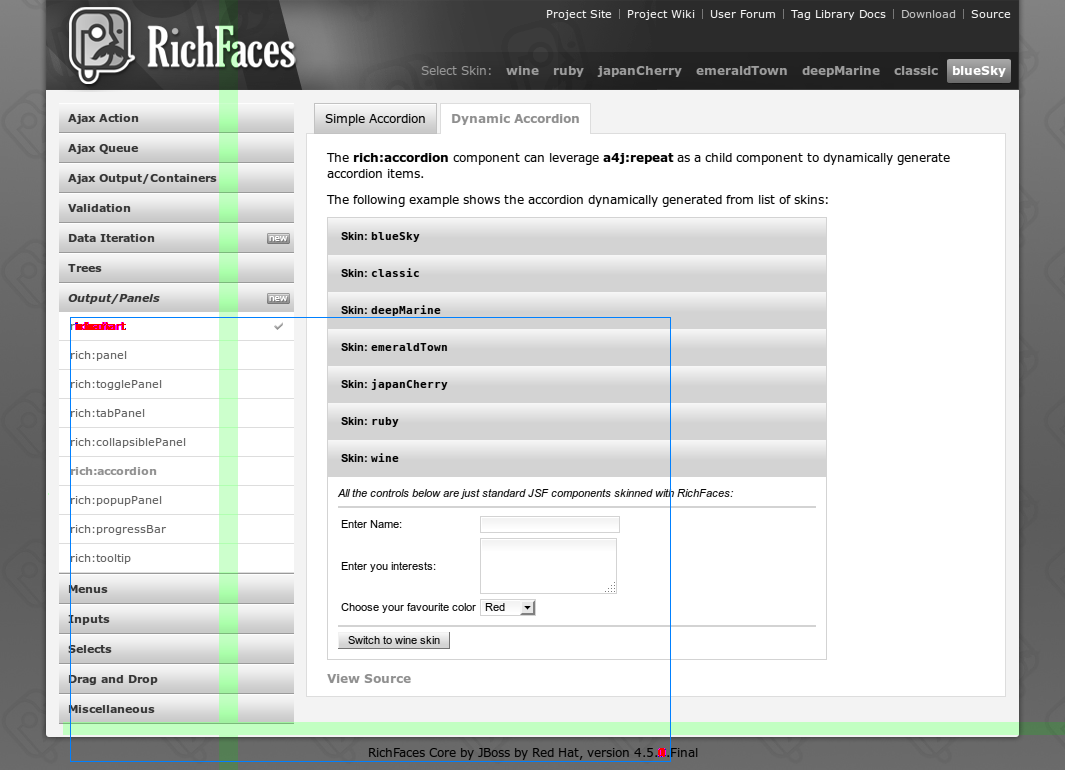
\includegraphics[width=1.0\textwidth]{figures/chartComponentRenamed.png}}}
      \end{center}
      \caption{RichFaces chart component renamed in application menu.}
      \label{fig:chartComponentRenamed}
  \end{figure*}
  
  \begin{figure*}[!htb]
      \begin{center}
      \leavevmode
      \centerline{\scalebox{1.0}{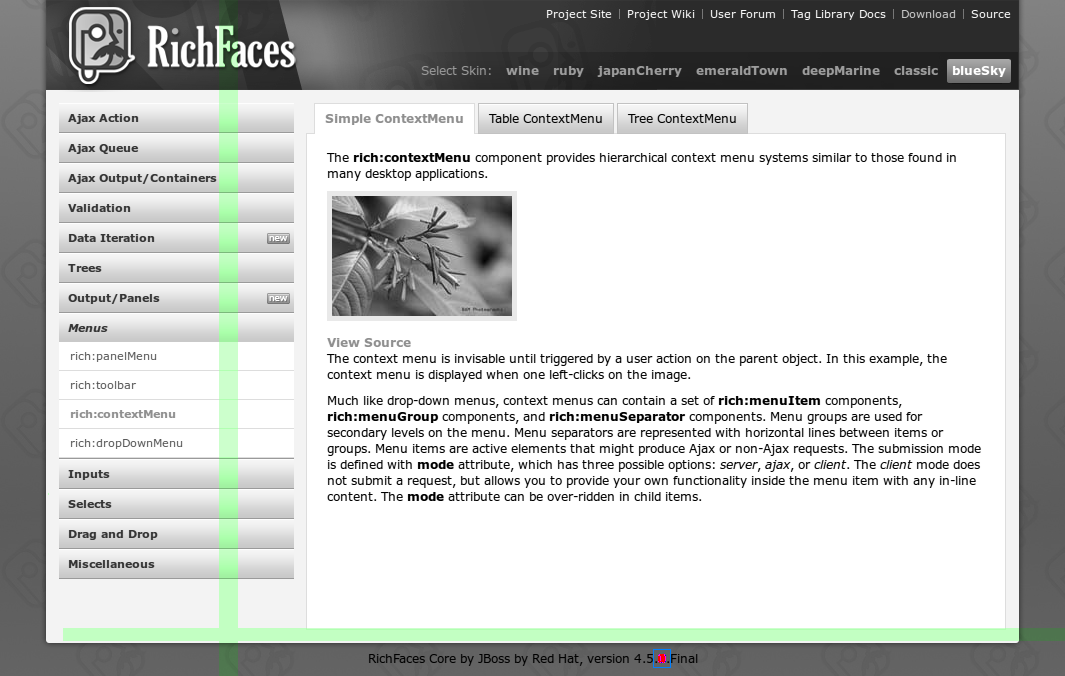
\includegraphics[width=1.0\textwidth]{figures/rchFacesVersionChanged.png}}}
      \end{center}
      \caption{RichFaces version changed after it was upgraded.}
      \label{fig:rfVersionChanged}
  \end{figure*}

  \section{Usage with CI}
    
  \section{Cloud ready}
  \label{sec:cloudReady}
  Improvement of effectiveness of a quality assurance team was our primary goal, when developing the tool. This include easy 
  deployment of the tool either in the organization infrastructure, or in a cloud environment. Particularly its web part, the
  Web manager for reviewing results (see \ref{sec:webManagerAppDesc}).
  
  We chose OpenShift open hybrid cloud by Red Hat, to proof the concept, that our solution is deployable to a cloud. One of the
  reasons is that it supports WildFly application server, which integrates well with ModeShape JCR repository \ref{chap:storage}.
  
  To login into the application\footnote{Application is available at 
  \url{http://jbosswildfly-jhuska.rhcloud.com/graphene-visual-testing-webapp}} one has to 
  use \texttt{LOGINNAME}, and password \texttt{PASSWORD}.
  
  Whole process of deploying Web Manager to OpenShift is described in Appendix \ref{appendix:e}. By following it, it is very easy
  to deploy the Web Manager application.
  
\chapter{Possible extensions}
\label{sec:plannedExtensions}
  
\chapter{Conclusion}
What I developed, What I improved, What can be better, Possible ways of extensions: OpenShift cartridge

\appendix
\chapter{Appendix A - GUI mockups of Web Manager UI}
\label{appendeix:a}

\begin{figure*}[!htb]
    \begin{center}
    \leavevmode
    \centerline{\scalebox{1.0}{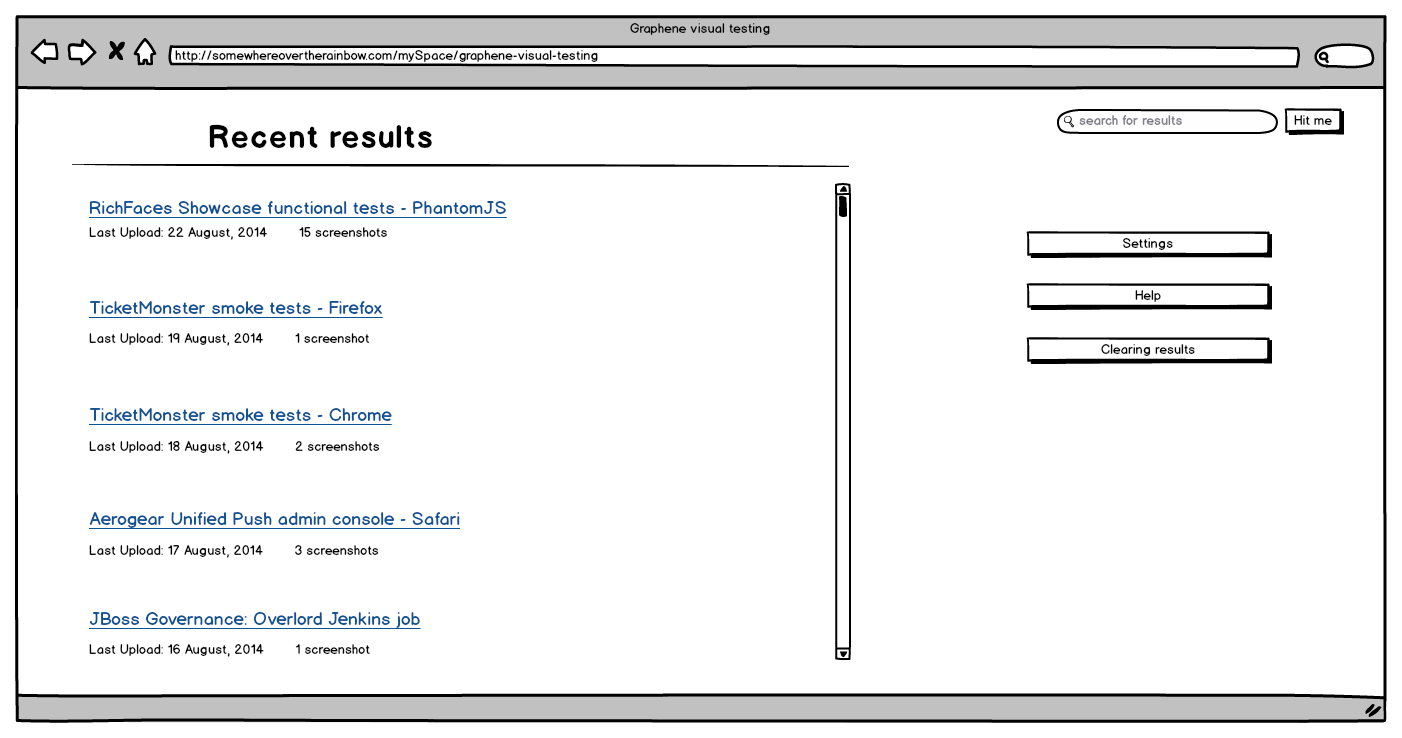
\includegraphics[width=1.0\textwidth]{figures/frontPage.png}}}
    \end{center}
    \caption{GUI mockup for result viewer web application - front page.}
    \label{fig:frontPageMock}
\end{figure*}

\begin{figure*}[!htb]
    \begin{center}
    \leavevmode
    \centerline{\scalebox{1.0}{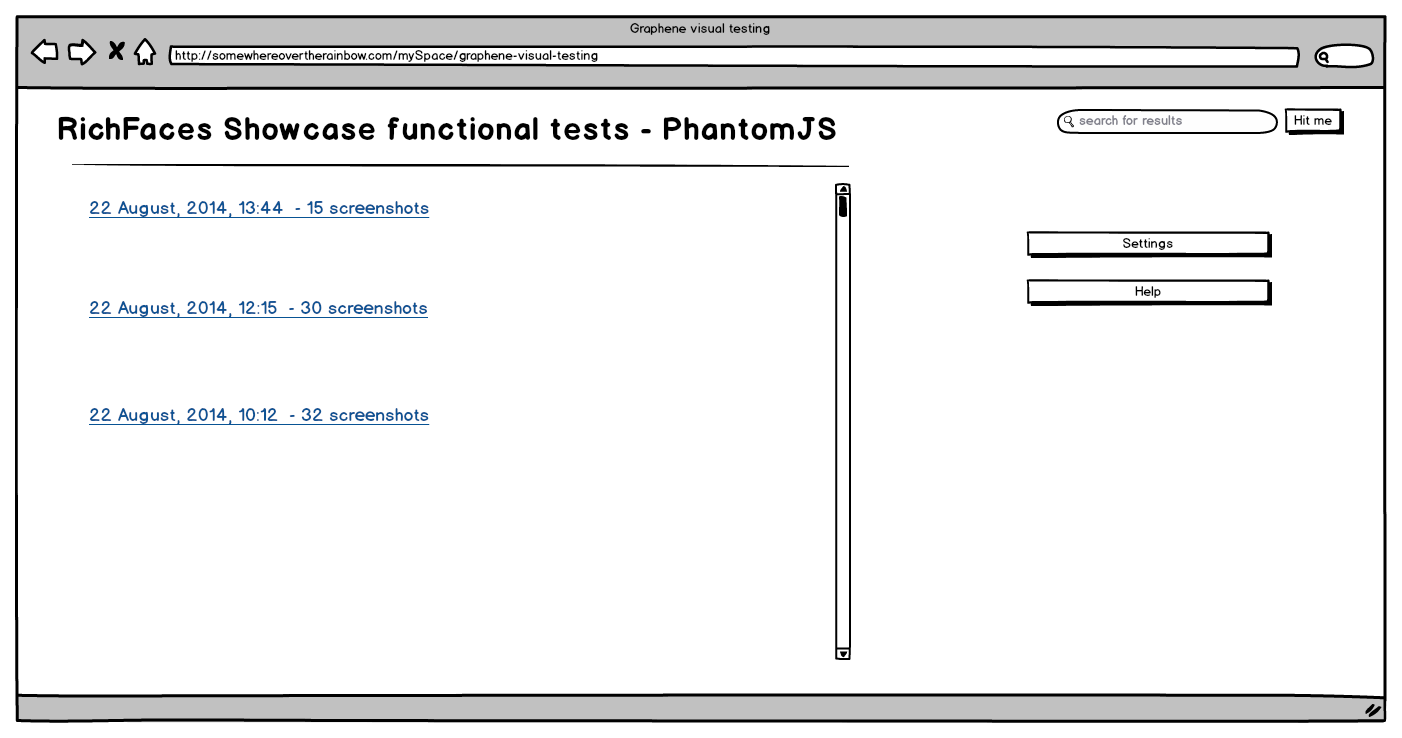
\includegraphics[width=1.0\textwidth]{figures/particularJob.png}}}
    \end{center}
    \caption{GUI mockup for result viewer web application - particular test suite run.}
    \label{fig:particularRunMock}
\end{figure*}

\begin{figure*}[!htb]
    \begin{center}
    \leavevmode
    \centerline{\scalebox{1.0}{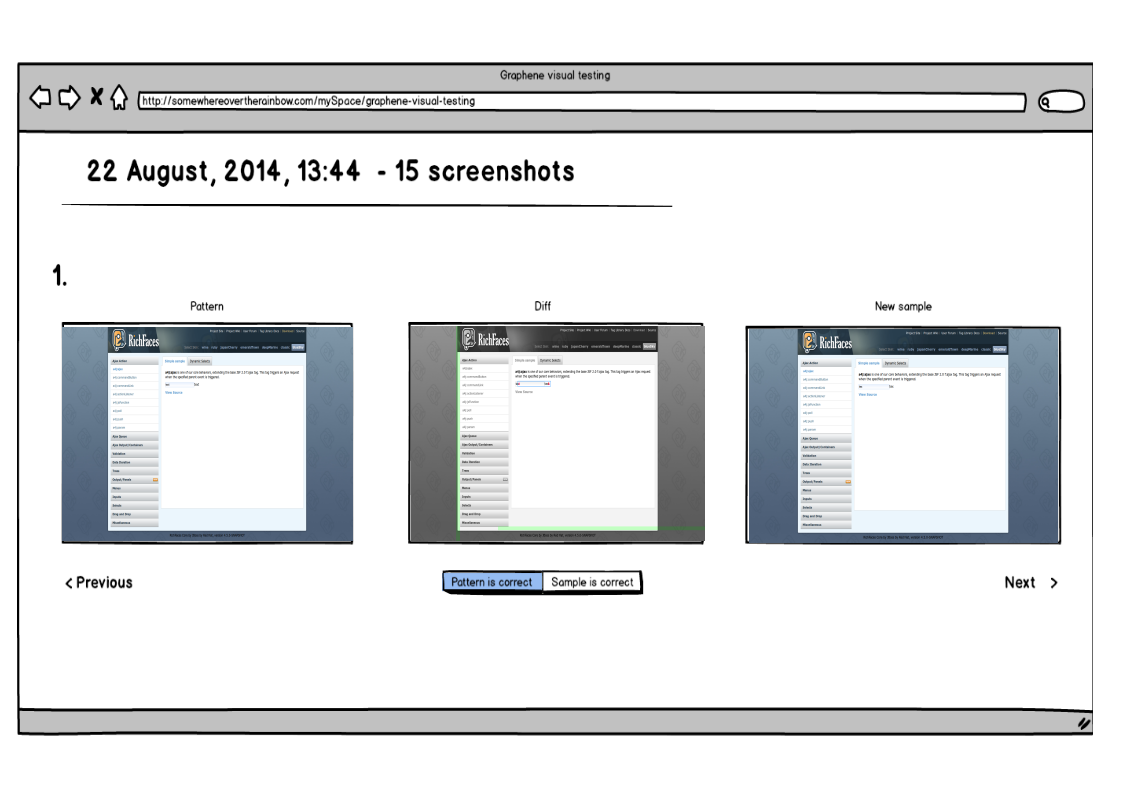
\includegraphics[width=1.0\textwidth]{figures/patternsSamplesDiffsAltered.png}}}
    \end{center}
    \caption{GUI mockup for result viewer web application - actual comparison results.}
    \label{fig:comparisonResultMock}
\end{figure*}

\chapter{Appendix B - List of contributions to opensource projects}
\label{appendix:b}
\begin{enumerate}
 \item Graphene visual testing arquillian extension
 \item Web Manager
 \item ESTE DOKONCIT: RUSHEYE to Arquillian, not merged yet
 \item RICHFACEs showcase test suite, not merged yet
 \item Graphene screenshooter, an extension to Graphene, which enables taking of the screenshots during functional testing.
       Available at: \url{https://github.com/arquillian/arquillian-graphene/tree/master/extension/screenshooter}.
 \item Add to Graphene Interceptors feature way to intercept in order. Feature request tracked with this issue:\\*
       \url{https://issues.jboss.org/browse/ARQGRA-423}.
\end{enumerate}


\chapter{Appendix C - Screenshots from Web Manager UI}
\label{appendix:c}
Screenshoty z web manazera.

\chapter{Appendix D - CD Attachment}
\label{appendix:d}
CD attachment popis

\chapter{Appendix E - How to deploy Web manager on OpenShift}
\label{appendix:e}
\begin{enumerate}
 \item Create an account at \url{https://www.openshift.com}
 \item Add application, under Java category, choose WildFly Application Server 8.2.0.Final
 \item Choose public URL, wished gear size (we used small), scaling options (we did not used scaling), region of your choice.
 \item Click in the created application from Applications menu.
 \item Add PostgreSQL database.
 \item Under remote access, find out the address to ssh into the application from command line.
 \item Run \texttt{wget \url{http://downloads.jboss.org/modeshape/4.1.0.Final/modeshape-4.1.0.Final-jboss-wf8-dist.zip}}
 \item Unzip the downloaded artifacts, and follow this 
    \url{https://docs.jboss.org/author/display/MODE40/Installing+ModeShape+into+Wildfly} tutorial to 
    enable Modeshape in WildFly installation.
 \item Clone the GIT repository of your application.
 \item Remove pre-generated \texttt{pom.xml}.
 \item Build and put \texttt{graphene-visual-testing-app.war} into deployments directory of the cloned repository.
 \item Alter the \texttt{standalone.xml} file, so it combines \texttt{standalone-modeshape.xml} and original \texttt{standalone.xml}.
 \item It should contains all necessary configurations for ModeShape. More information in the tutorial referenced in step 8.
 \item Commit and Push the changes into the remote Git repository.
 \item Your application should be available at the public URL of the application you created in OpenShift + add the end of the path:
 graphene-visual-testing-webapp
 \item The login and password to the application should be same as the ones for create WildFly user in step 8.
\end{enumerate}


\chapter{Appendix F}
\label{appendix:f}
Ako spustit samotne vizualne testovanie.

    % bibtex here
    \addcontentsline{toc}{chapter}{Bibliography}
    \pagestyle{plain}
    \bibliography{thesis}
    %[1] Hetzel, William C., The Complete Guide to Software Testing, 2nd ed. Publication info: Wellesley, Mass. : QED Information Sciences, 1988. ISBN: 0894352423.Physical description: ix, 280 p. : ill ; 24 cm.
    %[2] http://en.wikipedia.org/wiki/Waterfall_model
    %[3] http://en.wikipedia.org/wiki/Scrum_(software_development)
    %[4] http://www.w3schools.com/browsers/browsers_stats.asp
    %[5] http://en.wikipedia.org/wiki/Continuous_integration
    %[6] http://mogotest.com/
    %[7] https://github.com/BBC-News/wraith 
    %[8] http://phantomjs.org/
    %[9] http://en.wikipedia.org/wiki/WebKit
    %[10] http://slimerjs.org/
    %[11] http://en.wikipedia.org/wiki/Localhost
    %[12] http://media.tumblr.com/c5bf7caefde043ee7532b641c7f0e157/tumblr_inline_moaf774b5i1qz4rgp.jpg
    %[13] http://hop.ie/images/posts/wraith/example.png
    %[14] http://en.wikipedia.org/wiki/Facebook
    %[15] https://github.com/facebook/huxley
    %[16] http://en.wikipedia.org/wiki/JSON
    %[17] http://en.wikipedia.org/wiki/Software_as_a_service
    %[18] https://github.com/arquillian/arquillian-rusheye
    %[19] http://www.seleniumhq.org/docs/05_selenium_rc.jsp
    %[20] http://casperjs.org/
    %[21] https://is.muni.cz/auth/th/359345/fi_b/
    %[22] https://github.com/jjamrich/arquillian-rusheye
    %[23] http://richfaces.jboss.org/
    %[24] https://developer.jboss.org/thread/248301
    %[25] http://docs.oracle.com/javase/tutorial/sound/SPI-intro.html
    %[26] https://code.google.com/p/selenium/wiki/PageObjects
    %[27] https://docs.jboss.org/author/display/ARQGRA2/Page+Fragments
    %[28] http://stackoverflow.com/a/3751
    %[29] https://docs.jboss.org/author/display/MODE40/Why+use+a+repository
    %[30] https://is.muni.cz/auth/th/207442/fi_b/

\end{document}